%%% Template originaly created by Karol Kozioł (mail@karol-koziol.net) and modified for ShareLaTeX use

\documentclass[letterpaper,10pt]{article}
\usepackage[letterpaper]{geometry}
\usepackage{url}
\usepackage[T1]{fontenc}
\usepackage[utf8]{inputenc}
\usepackage{graphicx}
\usepackage{xcolor}
\usepackage{url}
\renewcommand\familydefault{\sfdefault}
\usepackage{tgheros}
\usepackage[defaultmono]{droidmono}

\usepackage{amsmath,amssymb,amsthm,textcomp}
\usepackage{enumerate}
\usepackage{multicol}
\usepackage{tikz}
\usepackage{float}

\DeclareMathOperator*{\argmin}{argmin}
\DeclareMathOperator*{\argmax}{argmax}
\DeclareMathOperator{\dash}{-}

\usepackage{geometry}
\geometry{total={210mm,297mm},
left=25mm,right=25mm,%
bindingoffset=0mm, top=20mm,bottom=20mm}


\linespread{1.3}

\newcommand{\linia}{\rule{\linewidth}{0.5pt}}

% custom theorems if needed
\newtheoremstyle{mytheor}
    {1ex}{1ex}{\normalfont}{0pt}{\scshape}{.}{1ex}
    {{\thmname{#1 }}{\thmnumber{#2}}{\thmnote{ (#3)}}}

\theoremstyle{mytheor}
\newtheorem{defi}{Definition}

% my own titles
\makeatletter
\renewcommand{\maketitle}{
\begin{center}
\vspace{2ex}
{\huge \textsc{\@title}}
\vspace{1ex}
\\
\linia\\
\@author \hfill \@date
\vspace{4ex}
\end{center}
}
\makeatother
%%%

% custom footers and headers
\usepackage{fancyhdr}
\pagestyle{fancy}
\lhead{}
\chead{}
\rhead{}
\lfoot{Assignment 1}
\cfoot{}
\rfoot{Page \thepage}
\renewcommand{\headrulewidth}{0pt}
\renewcommand{\footrulewidth}{0pt}
%

% code listing settings
\usepackage{listings}
\lstset{
    language=Python,
    basicstyle=\ttfamily\small,
    aboveskip={1.0\baselineskip},
    belowskip={1.0\baselineskip},
    columns=fixed,
    extendedchars=true,
    breaklines=true,
    tabsize=4,
    prebreak=\raisebox{0ex}[0ex][0ex]{\ensuremath{\hookleftarrow}},
    frame=lines,
    showtabs=false,
    showspaces=false,
    showstringspaces=false,
    keywordstyle=\color[rgb]{0.627,0.126,0.941},
    commentstyle=\color[rgb]{0.133,0.545,0.133},
    stringstyle=\color[rgb]{01,0,0},
    numbers=left,
    numberstyle=\small,
    stepnumber=1,
    numbersep=10pt,
    captionpos=t,
    escapeinside={\%*}{*)}
}

%%%----------%%%----------%%%----------%%%----------%%%

\begin{document}

\begin{titlepage}

\newcommand{\HRule}{\rule{\linewidth}{0.5mm}} % Defines a new command for the horizontal lines, change thickness here

\center % Center everything on the page
 
%----------------------------------------------------------------------------------------
%	HEADING SECTIONS
%----------------------------------------------------------------------------------------

\textsc{\LARGE University of Sydney}\\[1.5cm] % Name of your university/college

\textsc{\Large Machine Learning and Data Mining}\\[0.5cm] % Major heading such as course name
%\textsc{\large Minor Heading}\\[0.5cm] % Minor heading such as course title

%----------------------------------------------------------------------------------------
%	TITLE SECTION
%----------------------------------------------------------------------------------------

\HRule \\[0.4cm]
{ \huge \bfseries Classification Task}\\[0.4cm] % Title of your document
\textsc{\Large Assignment 1}\\[0.5cm]
\HRule \\[1.5cm]
 
%----------------------------------------------------------------------------------------
%	AUTHOR SECTION
%----------------------------------------------------------------------------------------

\begin{minipage}{0.4\textwidth}
\begin{flushleft} \large
\emph{Authors:}\\
\textsc{Tinju Abraham\\		
		Claudio Aracena\\
		Rafael Possas} % Your name
\end{flushleft}
\end{minipage}
~
\begin{minipage}{0.4\textwidth}
\begin{flushright} \large
\emph{Lecturers:} \\
 \textsc{Fabio Ramos\\
 		 Roman Marchant} % Supervisor's Name
\end{flushright}
\end{minipage}\\[4cm]

% If you don't want a supervisor, uncomment the two lines below and remove the section above
%\Large \emph{Author:}\\
%John \textsc{Smith}\\[3cm] % Your name

%----------------------------------------------------------------------------------------
%	DATE SECTION
%----------------------------------------------------------------------------------------

{\large \today}\\[3cm] % Date, change the \today to a set date if you want to be precise

%----------------------------------------------------------------------------------------
%	LOGO SECTION
%----------------------------------------------------------------------------------------


\includegraphics[width=0.5\textwidth]{university-of-sydney-logo}\\[1cm] % Include a department/university logo - this will require the graphicx package
 
%----------------------------------------------------------------------------------------

\vfill % Fill the rest of the page with whitespace

\end{titlepage}

\begin{abstract}
Categorization of large documents is one of the areas where Natural Language Processing can be used to create models that can help to predict different features of a text. The first step for applying such models would be to create a VSM (Vector Space Model) where the words of the given description could be represented as numbers. Hence, a predictive algorithm would be able to process the text as a matrix, usually with a very high number of dimensions, and predict the possible outcome according to the data provided. As the data could be considered of very high dimensions, some pre-processing and feature extractions techniques are needed to make the algorithm faster when running on a computer. This work comprises of trying to predict a category of a given application through its text description. The outcome can be very useful for processing text in application stores like Play Store and Apple store since the amount of data increases every day along with the needs to better categorize the applications in their correct genre. One of the goals was to evaluate the performance of different algorithms using a third party machine learning library and to implement the one that would perform the best in the given dataset. The logistic regression was the algorithm of choice as it had the best overall metrics / results across all tested algorithms. In depth analysis of the results and implementation of the algorithm will be provided in this work along with a brief discussion of future work.
\end{abstract}

\section{Introduction}

Supervised Learning is one of the main approaches of Machine Learning. Classification is an instance of supervised learning, where the goal is to learn a mapping from inputs $x$ to outputs $y$, where $y \in \{1, 2, 3, . . . , C\}$, with $C$ being the number of classes.

The aim of this classification task is to learn to classify unlabelled test data (predict the category) which consists of the features without class names/labels. The task should be solved by taking the training set which consists of large set of labelled training set and building a classifier from those instances. The Classifier would then able to classify the unlabelled examples based on the information learned from the training set. 

\begin{figure}[H]
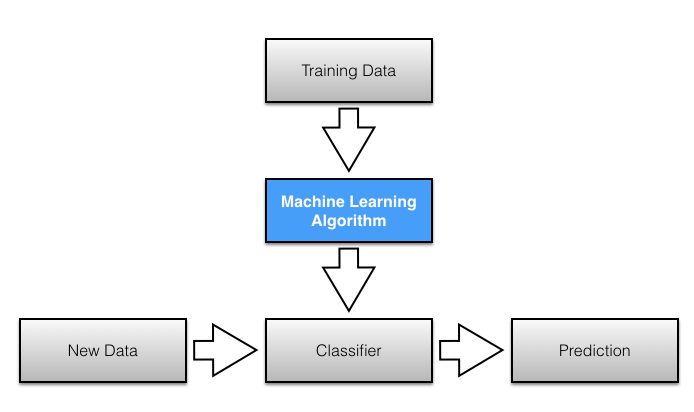
\includegraphics[width=0.8\textwidth]{learning_algorithm_1}
\centering
\caption{Image Source: Raschka, S. (2014). Naive Bayes and Text Classification I-Introduction and Theory.}
\label{fig:1}
\end{figure}

In machine learning, the observations are often known as instances, the explanatory variables are termed features and the possible categories to be predicted are classes. The information related to the classification task explored in this report are given below.

\textbf{Instances}: A training set with 20,104 rows each corresponding to an app

\textbf{Features}: Training set has 13,626 columns each corresponding to tf-idf values which are extracted from words in the description of each app. If a word is found in the description of an app, it has a tf-idf value. On the other hand, its tf-idf value is zero if the word is not found in the description of the app.

In information retrieval, tf–idf is frequency–inverse document frequency,  a numerical statistic that is intended to reflect how important a word is to a document in a collection or corpus. The tf-idf value increases proportionally to the number of times a word appears in the document, but is offset by the frequency of the word in the corpus, which helps to adjust for the fact that some words appear more frequently in general~\cite{wiki:tfidf}.

\textbf{Classes}: The training set has labels associated with each row. There are 30 labels or classes associated with the apps. The test data should be labeled into these categories by the classifier.  

\section{Methods}

This section discusses the methods explored to deal with the challenges of high dimensional data and the theoretical aspects of the classifier used for classification task. Also, the implementation of the objective function of the classifier for training the dataset is illustrated.

\subsection{Exploratory Data Analysis (EDA)}

Before starting any data manipulation, it is a good practice and an effective way to extract insights about the data to do an exploratory data analysis. This process is about detecting and describing patterns, trends, and relations in data, motivated by certain purposes of investigation~\cite{andrienko2006exploratory}, often with visual methods. 

In the case of this assignment a good question to answer is how the labels are distributed in all 30 categories. To extract this kind of information the use of a histogram is suitable. The figure~\ref{fig:2} shows the histogram of the frequency of categories.

\begin{figure}[H]
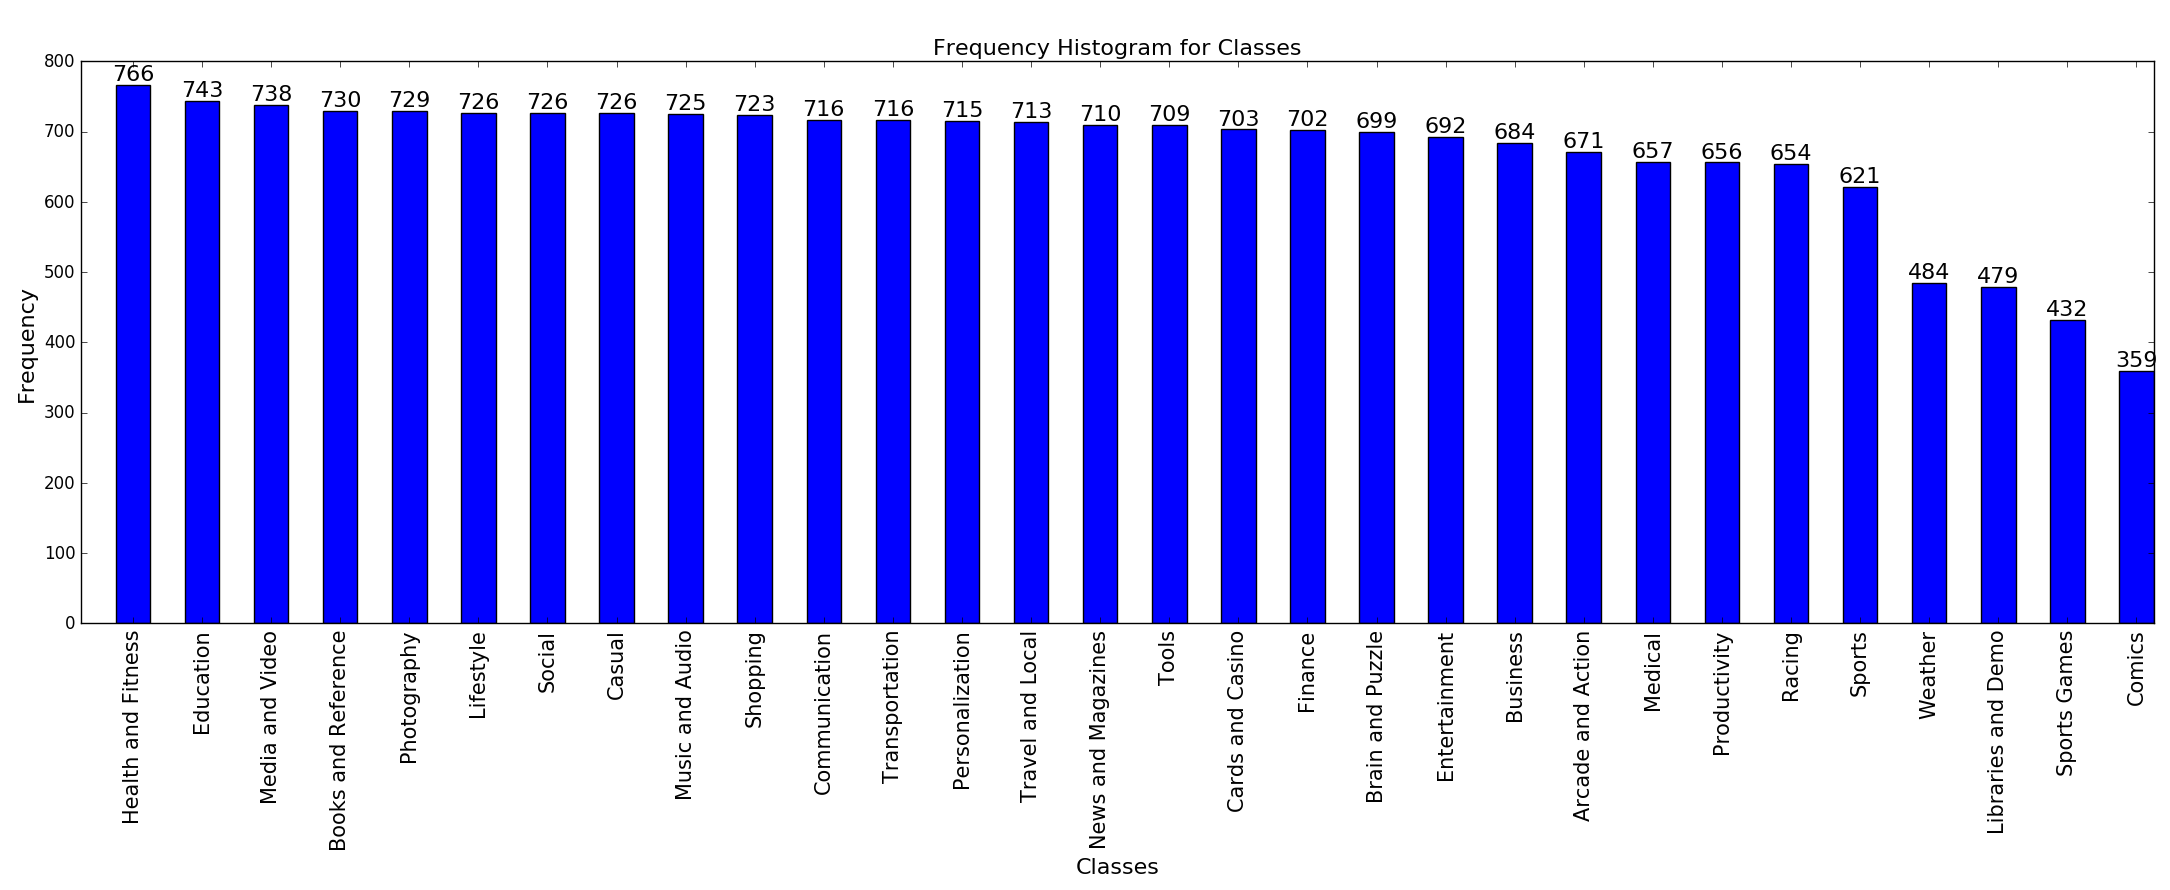
\includegraphics[width=\textwidth]{histo}
\centering
\caption{Frequency Histogram for classes in the dataset}
\label{fig:2}
\end{figure}

It is possible to observe that there is a equitable distribution among almost all categories with a frequency range from 621 to 766 instances. However, there are four categories which their frequencies are lower than the rest with a range from 359 to 484.

\subsection{Pre-processing}

Machine learning algorithms learn from data. It is critical to feed them the right data for the problem it needs to solve. Even if the data provided is good, it is needed to make sure that it is in a useful scale, format and even meaningful features are included.

Dimensionality reduction is the process of converting a set of highly dimensional data into a set with lesser dimensions~\cite{russell1995modern}. This reduction not only helps in the processing needs for running the algorithm but also reveals latent variables in the data~\cite{bishop2007pattern}. In most cases, applying these methods can help in solving machine learning problems as it obtains better features for classification or regression algorithms.

The set given for this task can be categorized as highly dimensional if we put every word in our vocabulary as a feature to be processed by our algorithm. There are 13,026 words in total, however, each application description only uses a few of those words, therefore, making our dataset sparse. For this work PCA (Principal Component Analysis) was used as a dimensionality reduction option. PCA is a technique for taking a dataset and reducing its dimensions by finding the direction in which the tuples line up best~\cite{rajaraman2012mining}. The first principal component is that where the variance is the higher as it can be illustrated in the Figure~\ref{fig:3}.

\begin{figure}[H]
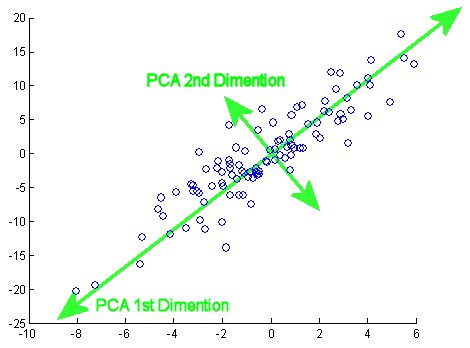
\includegraphics[width=0.7\textwidth]{pca}
\centering
\caption{Principal Component Analysis (PCA) example}
\label{fig:3}
\end{figure}

%Looking at the data also helps to identify some other pre-processing techniques. For instance, the most frequent features (sum on column) were removed, as they could be seen as “stop-words” in the text and, therefore, would not contribute too much for predicting the document category. The dataset went from 13.626 features to 13.048 after applying the aforementioned pre-processing technique. The Figure~\ref{fig:4} illustrates the pipeline of the entire pre-processing stage.

%\begin{figure}[H]
%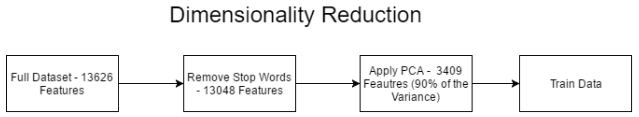
\includegraphics[width=0.7\textwidth]{pre-processing}
%\centering
%\caption{Dimensionality Reduction process}
%\label{fig:4}
%\end{figure}

\subsection{Classifier}

The term Classifier refers to the classification algorithm that maps an unlabeled instance into a category or class. The classifier’s evaluation is most often based on the accuracy of the prediction. The algorithm implemented for classification of the test data is explained below. For this work, Logistic Regression was implemented as it gave us the best accuracy when running the dataset with a 10-fold cross validation.

\subsubsection{Logistic Regression}

Logistic regression sometimes called the logistic model or logit model, analyzes the relationship between multiple independent variables and a categorical dependent variable, and estimates the probability of occurrence of an event by fitting data to a logistic curve~\cite{park2013introduction}. It is based on the below discriminative model for binary classification.

\begin{gather}
p(y|\boldsymbol{x},\boldsymbol{w}) = Ber(y|\sigma(\eta)) = \sigma(\eta)^{y}(1 - \sigma(\eta))^{1-y} \\
\eta = \boldsymbol{w}^{T}\boldsymbol{x}
\end{gather}

$\sigma(\eta)$ refers to the sigmoid function, also known as the logistic or logit function. The term “sigmoid” means S-shaped. It is also known as a squashing function, since it maps the whole real line to [0,1], which is necessary for the output to be interpreted as a probability. This is defined as 

\begin{equation}
\sigma(\eta) = \frac{1}{1 + exp(-\eta)} = \frac{e^{\eta}}{e^{\eta} + 1}
\end{equation}

Putting these two steps together we get $p(y|\boldsymbol{x},\boldsymbol{w}) = Ber(y|\sigma( \boldsymbol{w}^{T}\boldsymbol{x}))$.This is called logistic regression due to its similarity to linear regression~\cite{murphy2012machine}. 
In logistic regression training, weights are set to maximize the Conditional Log Likelihood(CLL).

\begin{equation}
\boldsymbol{W} \leftarrow \argmax_{W} \sum_{d \in D} \ln P(Y^d|X^d, W)
\end{equation}

To prevent overfitting, regularization can be used by penalizing large weights by changing the training objective:

\begin{equation}
\boldsymbol{W} \leftarrow \argmax_{W} \sum_{d \in D} \ln P(Y^d|X^d, W) - \frac{\lambda}{2}\parallel W \parallel^2 
\end{equation}

Where $\lambda$ is a constant that determines the amount of smoothing. 

\subsection{Implementation}

The implementation details of the classifier are described in this subsection.

\textbf{Optimization process}

To find the minimum value of the cost function an optimization process was done. The chosen function for find the optimal weights was $fmin\_l\_bfgs\_b$ from scipy library. This function is based on Broyden–Fletcher–Goldfarb–Shanno algorithm, which is an iterative method for solving unconstrained nonlinear optimization problems~\cite{wiki:bfgs}. Moreover, this function is faster than its original approach ($fmin\_bfgs$), because it stores less calculations. 

To seize the availability of multiple cores in modern computers, the optimization process was implemented using the joblib library, which create several parallel jobs. Since for the multi-class Logistic Regression it is necessary to create binary classifiers, each job consists in train a specific binary classifier.

\textbf{Regularization} 

One technique that is often used to control the over-fitting phenomenon in such cases is that of regularization, which involves adding a penalty term to the cost function in order to discourage the coefficients from reaching large values~\cite{bishop2007pattern}.
To choose a regularization parameter lambda several values were tested in the Logistic Regression classifier. In the table~\ref{table:3} the resulting F-score values when a 10-fold cross-validation process for all the data with several values of lambda are showed.

\begin{table}[H]
\centering
\label{table:3}
\begin{tabular}{|c|c|}
\hline
\textbf{\begin{tabular}[c]{@{}c@{}}Regularization \\ parameter $\lambda$\end{tabular}} & \textbf{F-score} \\ \hline
0.03 & 64.4 \% \\ \hline
0.1 & 65.5 \% \\ \hline
0.3 & 65.9 \% \\ \hline
0.5 & 65.6 \% \\ \hline
1 & 65.4\% \\ \hline
\end{tabular}
\caption{F-score results for several regularization paramters ($\lambda$)}
\end{table} 

As the Table~\ref{table:3} shows there is no big difference among different regularization parameters, but the maximum is reached at 0.3, which it is the chosen value for the next experiments.

\section{Experiments and results}

In this section, the experiments conducted on classification algorithms and the results are discussed. Also the metrics and evaluation procedures to evaluate the accuracy and other measures of the results of the algorithms in different experiments are illustrated.

\subsection{Metrics} 

Evaluating performance of a classifier can be as easy as measuring its accuracy, however, this method can lead to misleading conclusions if used as the only driver. Accuracy is not the only metric for evaluating the effectiveness of a classifier. In this work, it was also introduced the precision, recall and f-score metrics as they tell different things about the data.

Precision (also called positive predictive value) is the fraction of retrieved instances that are relevant, while recall (also known as sensitivity) is the fraction of relevant instances that are retrieved. Both precision and recall are therefore based on an understanding and measure of relevance. Finally, the  F\-score conveys the balance between the precision and the recall~\cite{wiki:pandr}. The definitions of Precision, Recall and F\-score in classification context are given below.

\begin{gather}
Precision\ P\ = \frac{tp}{tp + fp} \\ 
Recall\ R\ = \frac{tp}{tp + fn} \\
Accuracy\ Acc\ = \frac{tp + tn}{tp + tn + fp + fn} \\
F \dash score\ F_{1}\ = \frac{2PR}{P+R}
\end{gather}

\subsection{Evaluation Procedure}

In order to prevent over fitting and better train the algorithm, the dataset was divided into disjoint training and cross-validation sets as illustrated in the figure~\ref{fig:5}

\begin{figure}[H]
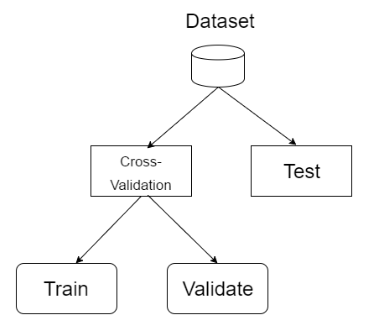
\includegraphics[width=0.5\textwidth]{procedure}
\centering
\caption{Learning Procedure}
\label{fig:5}
\end{figure}

In the simplest case, testing sets are constructed by splitting the original dataset into more than one part. However, evaluations obtained in this case tend to reflect the particular way the data are divided up. Statistical sampling helps to get more accurate measurements, which is known by cross-validation~\cite{kohavi1995study}.

The main goal of cross-validation is to ensure that every sampling from the original set has the probability of appearing in the training and testing set. The k-fold cross validation strategy is that where the original sample is randomly partitioned into k subsamples and one is left out each iteration~\cite{kohavi1995study}. In the cross validation evaluation procedure experimented in the classifier, 10\% of the given training dataset is taken as test data, the remaining 90\% data ( which is considered as the training data in that trial) has been used by the classifier to predict the classes of the test data and this procedure is repeated 10(k=10) times. The precision is calculated as the average of the 10 trials. The advantage is that every data point gets to be in a test set exactly once and this helps in the better evaluation of the method. The size of the test set and the number of trials can be chosen independently in a cross validation method.

This evaluation procedure is used only in the experiment and is not called as a procedure in the final implementation of the objective function. 

\subsection{Experiments}

All the experiments were done using the Cross Validation with 10 folds and the metrics precision, recall, accuracy, F1 Score and execution time were extracted as the Tables~\ref{table:1}~and~\ref{table:2} show. The tests were divided into the set with minimal dimensionality reduction (only stop words) and a set with full dimensionality reduction (pca + stop words). All the algorithms except from Logistic Regression where extracted from sklearn library for benchmarking purposes.

\begin{table}[H]
\centering
\label{table:1}
\begin{tabular}{|l|c|c|c|c|c|}
\hline
\multicolumn{1}{|c|}{\textbf{Algorithm}} & \textbf{Precision / STD (\%)} & \textbf{Recall / STD (\%)} & \textbf{F-Score / STD (\%)} & \textbf{Accuracy (\%)} & \textbf{Time (s)} \\ \hline
\textbf{\begin{tabular}[c]{@{}l@{}}Logistic \\ Regression\end{tabular}} & 65.62 $\pm$ 1.28 & 66.37 $\pm$ 1.30 & 65.37 $\pm$ 1.28 & 65.34 & 1953 \\ \hline
\textbf{\begin{tabular}[c]{@{}l@{}}Gaussian \\ Naïve Bayes\end{tabular}} & 44.33 $\pm$ 1.11 & 45.09 $\pm$ 1.25 & 44.29 $\pm$ 1.13 & 44.32 & 99 \\ \hline
\textbf{\begin{tabular}[c]{@{}l@{}}Multinomial \\ Naïve Bayes\end{tabular}} & 61.94 $\pm$ 0.72 & 65.70 $\pm$ 0.93 & 61.14 $\pm$ 0.75 & 60.11 & 17 \\ \hline
\textbf{KNN} & 33.57 $\pm$ 1.67 & 55.46 $\pm$ 2.47 & 38.07 $\pm$ 1.95 & 45.23 & 7091 \\ \hline
\end{tabular}
\caption{Metrics for 10 fold Cross Validation without PCA}
\end{table}

\begin{table}[H]
\centering
\label{table:2}
\begin{tabular}{|l|c|c|c|c|c|}
\hline
\multicolumn{1}{|c|}{\textbf{Algorithm}} & \textbf{Precision / STD (\%)} & \textbf{Recall / STD (\%)} & \textbf{F-Score / STD (\%)} & \textbf{Accuracy (\%)} & \textbf{Time (s)} \\ \hline
\textbf{\begin{tabular}[c]{@{}l@{}}Logistic \\ Regression\end{tabular}} & 61.41 $\pm$ 0.75 & 60.88 $\pm$ 0.75 & 59.98 $\pm$ 0.74 & 61.69 & 2873 \\ \hline
\textbf{\begin{tabular}[c]{@{}l@{}}Gaussian \\ Na\"{i}ve Bayes\end{tabular}} & 14.90 $\pm$ 1.07 & 31.35 $\pm$ 1.72 & 15.38 $\pm$ 1.04 & 22.34 & 646 \\ \hline
\textbf{\begin{tabular}[c]{@{}l@{}}Multinomial \\ Na\"{i}ve Bayes\end{tabular}} & NA & NA & NA & NA & NA \\ \hline
\textbf{KNN} & 39.68 $\pm$ 1.03 & 56.00 $\pm$ 1.34 & 43.57 $\pm$ 0.82 & 44.38 & 2012 \\ \hline
\end{tabular}
\caption{Metrics for 10 fold Cross Validation with PCA}
\end{table}

\subsection{Extensive Analysis}

From experiments subsection we can observe that the best results are obtained with Logistic Regression without dimensionality reduction. This was one of the main reasons to choose Logistic Regression as the final algorithm to predict labels in the test data. 

As it is described in the Methods section, Logistic Regression is an algorithm that can be implemented easily, being one of its best advantages. However, when it is used in big datasets the training time could be considerable. In our experiments this algorithm tested using 10 fold cross-validation have a execution time of around 30 minutes, and around 15 minutes longer if PCA is applied to the dataset. 

Some alternatives to Logistic Regression could be Multinomial Na\"{i}ve Bayes, K-Nearest Neighbour (KNN) and Gaussian Na\"{i}ve Bayes. The first one have a low execution time, but its implementation could be considered complex given the way is implemented in sklearn. A simple implementation of Multinomial Naive Bayes generates increments in execution time. The second option (KNN) shows worse results and high execution times, however it is also an algorithm of simple implementation. Lastly, Gaussian Na\"{i}ve Bayes shows the worst performance among all the options, even though its simple implementation and fast execution are its main advantages.

During the experiments, dimensionality reduction as pre-processing was tested. One may think this kind of techniques can help to reduce noise and help to improve the results. However, the performance and execution time of all algorithms were worse or equal after applying the pre-processing pipeline described in Methods section. Some reasons to explain this behaviour could be that the reduction of features using PCA could remove unique features for classes and trying to keep more general features, losing the capability of identifying more specific cases.    

\subsubsection{Confusion Matrix}

A Confusion Matrix is a specific table layout that allows visualization of the performance of an algorithm. Each column of the matrix represents the instances in a predicted class while each row represents the instances in an actual class (or vice-versa)~\cite{wiki:confusion}.

In order to check where the Logistic Regression classifier is making wrong predictions a small experiment was done. Randomly 1/3 of the training data was using for testing and the rest for training. From the predicted labels and the testing labels a confusion matrix was done to check which classes are being confused by the classifier. Figure~\ref{fig:4} shows the resulting confusing matrix.

\begin{figure}[H]
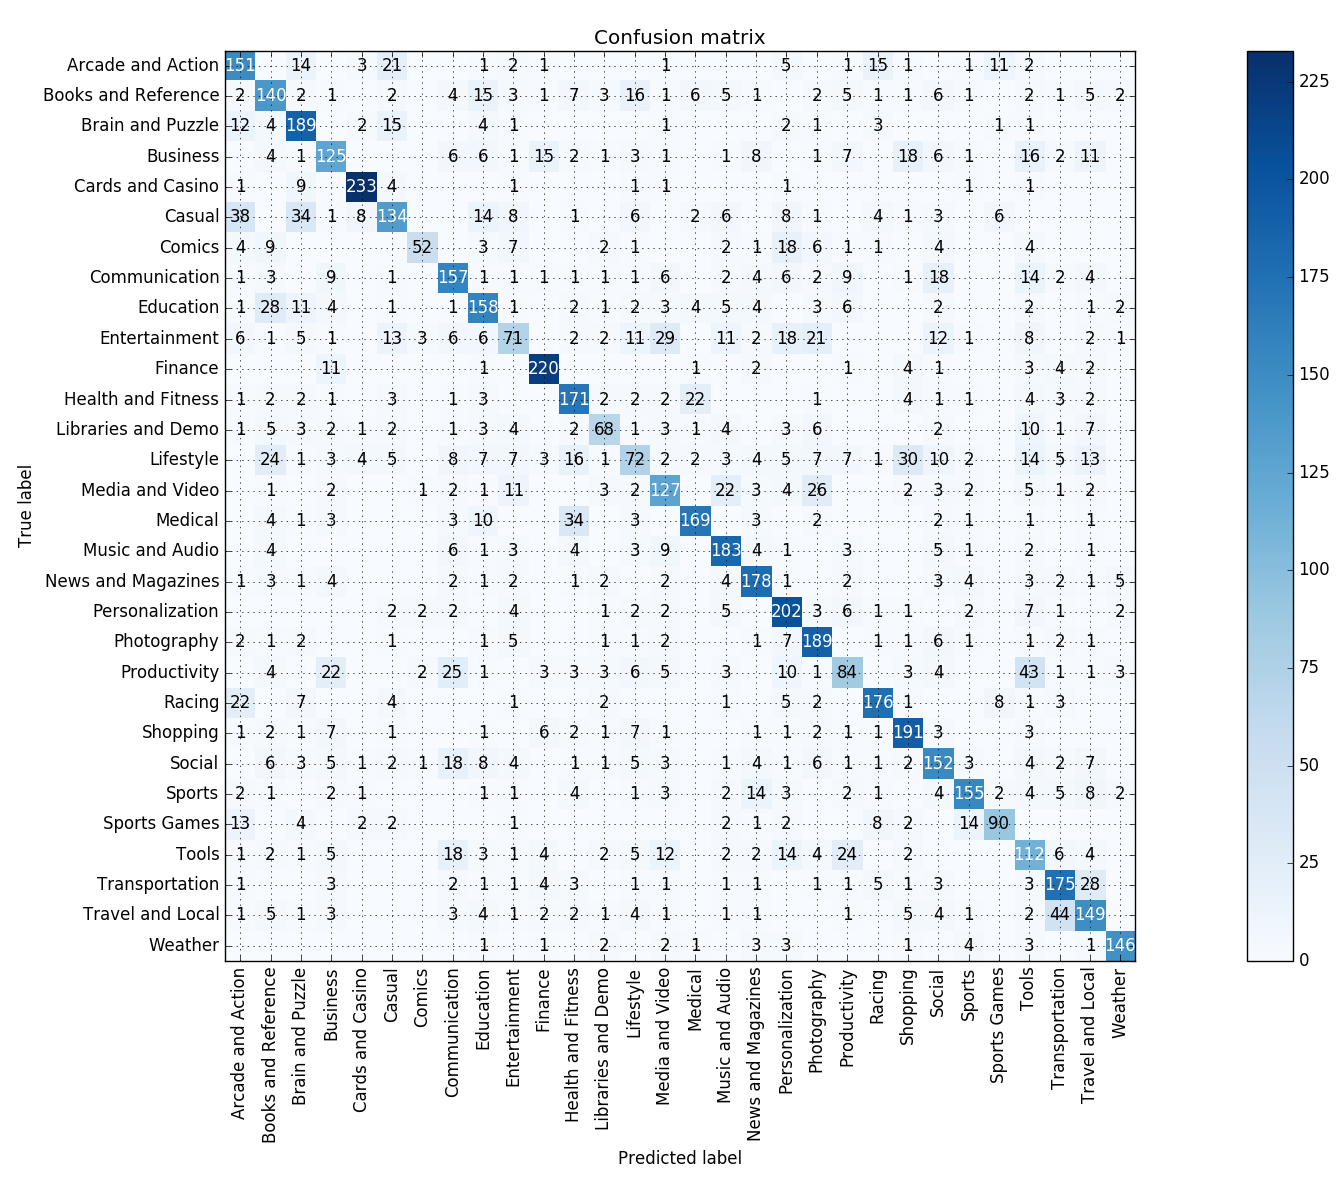
\includegraphics[width=\textwidth]{cm}
\centering
\caption{Confusion Matrix Sample}
\label{fig:4}
\end{figure}

From the matrix, it is possible to observe that a big part of the instances are being classified correctly (shown in the diagonal of the confusion matrix). However, some classes are being confused such as \textit{Tools}, \textit{Business}, \textit{Communication} and \textit{Productivity}; \textit{Book and Reference}, \textit{Brain and Puzzles} and \textit{Education}; \textit{Entertainment}, \textit{Media and Video}, \textit{Music and Video} and \textit{Photography}; \textit{Transportation} and \textit{Travel and Local}. Looking into the confused categories it is possible to notice they describe similar classes of applications and probably the words (features) to represent their functionality are similar. This property of the data is one of the main reasons why the classifier can not predict with high performance for those categories.    

\section{Discussion}

While doing the classification task, the strategy was to do a comparison study of performance and accuracy using the existing packages of classification and then implement the objective function. In general, the following challenges were faced during the entire process.

Curse of dimensionality – When the number of dimension grows, the volume of the space increases so fast that the available data becomes sparse. The complexity of many classification algorithms is exponential with respect to the number of dimensions. Some of the algorithms tried in this experiment performed really bad because of this dimensionality issue. Few algorithms which we had to drop because of poor performance are listed below
Xgboost – Poor performance that we had to drop experimenting with the algorithm.
GradientBoostClassifier
Random forest 

Dimensionality Reduction


Combining different algorithms - After a better understanding of the strengths and limitations of each method, we wanted to investigate the possibility of integrating two or more algorithms in the classifier to utilize the strengths of one method to complement the weaknesses of another. Considering the huge dataset and the computational performance, it was difficult to do more experiments to come up with a feasible solution within the limited time of the assignment task.


\section{Conclusions and future work}

Few tasks that were not feasible in the limited time for the classification assignment, which we would like to try in future:

Would combining unrelated algorithms which were well performing and giving accurate results yield a better result?

Which feature selection methods are high performing and scalable across different classifiers in the mentioned classification task? 


\nocite{wiki:fscore}
\nocite{wiki:pandr}
\nocite{wiki:stat} 
\nocite{wiki:curse}
%biblio
\bibliographystyle{unsrt}
\bibliography{biblio}

\section{Appendix}
\begin{lstlisting}[label={list:first},caption=Class Definition]
import numpy as np
from scipy.optimize import fmin_l_bfgs_b
from joblib import Parallel, delayed
import multiprocessing

class LogisticRegression:
    def __init__(self):
        print("Logistic Regression Class created")
        self.all_theta = []
        self.list_classes = []
\end{lstlisting}

\begin{lstlisting}[label={list:second},caption=Sigmoid Function]
	def sigmoid(self, X):
		return 1 / (1 + np.exp(-X))
\end{lstlisting}

\begin{lstlisting}[label={list:third},caption=Cost Function]
	def cost_function_reg(self, theta, X, y, l):
        m, n = X.shape
        J = (1/m) * (-y.T.dot(np.log(self.sigmoid(X.dot(theta)))) \ 
        	- (1-y.T).dot(np.log(1 - self.sigmoid(X.dot(theta))))) \
            + (l/m)* 0.5 * theta[1:].T.dot(theta[1:])
        return J
\end{lstlisting}

\begin{lstlisting}[label={list:fourth},caption=Gradient Function]
    def grad_function_reg(self, theta, X, y, l):
        m, n = X.shape
        grad = (1/m) * X.T.dot(self.sigmoid(X.dot(theta)) - y)
        grad[1:] = grad[1:] + (l/m)*theta[1:]
        return grad
\end{lstlisting}

\begin{lstlisting}[label={list:fifth},caption=Training Process]
    def fit(self, X, y, l):
        self.list_classes = list(set(y))
        self.list_classes.sort()

        classes = len(self.list_classes)
        X = self.add_theta0(X)
        num_cores = multiprocessing.cpu_count() -1
        results = Parallel(n_jobs=num_cores) 
        		  (delayed(self.logistic_train_one_class)
        		  (X, y, self.list_classes, l, c) for c in range(classes))
        self.all_theta = np.asarray(results)

    def logistic_train_one_class(self, X, y, list_classes, l, c):
        m, n = X.shape
        initial_theta = np.zeros(n)
        y_class = self.get_y_class(y, list_classes, c)

        def decorated_cost(theta):
            return self.cost_function_reg(theta, X, y_class, l)

        def decorated_grad(theta):
            return self.grad_function_reg(theta, X, y_class, l)

        theta = fmin_l_bfgs_b(decorated_cost, initial_theta, maxiter=50, 
                fprime=decorated_grad)
        return theta[0]
\end{lstlisting}

\begin{lstlisting}[label={list:fifth},caption=Prediction Process]
    def predict(self, X):
        m, n = X.shape
        X = self.add_theta0(X)
        y_pred = []
        for i in range(m):
            max_index = np.argmax(self.sigmoid(
            			self.all_theta.dot(np.transpose(X[i, :]))))
            y_pred.append(self.list_classes[max_index])
        return y_pred
\end{lstlisting}


\end{document}
